\section{Fase 4: Análisis Exploratorio de datos oncológicos}

En esta fase, el científico de datos obtiene el conjunto de datos o imágenes que fueron organizados previamente por el ingeniero de datos y realiza un \textit{Análisis exploratorio de datos} para descubrir patrones generales en la información generada. Cabe resaltar, que en esta fase el acompañamiento del medico experto en oncología es de vital importancia, ya que los datos o imágenes que van ser explorados por el científico pueden contener variables que pueden tener o no un valor significativo para el experto, ayudando así a determinar si el análisis planteado para responder la pregunta va o no por un buen camino, de modo que es posible que se agreguen o eliminen diversas variables para lograr el resultado esperado. Adicionalmente, es necesario que los diversos análisis generados estén apoyados con gráficas que sean entendibles por todo el \textit{Data Analysis Team}, esto con el proposito de aportar ideas, y desde esta fase ir encontrando posibles correlaciones entre las variables oncológicas.

Se debe agregar, que en esta fase se abarcan todas las actividades para construir el conjunto de datos o imágenes que se utilizará en la siguiente etapa de modelado y ejecución. Entre las actividades se encuentran el procesamiento y transformación de datos oncológicos, en donde es necesario realizar la limpieza de datos, combinar datos de múltiples fuentes y transformar los datos en variables de valor. En esta fase, es importante el trabajo en equipo y la comunicación continua entre el ingeniero y el científico de datos para tratar los valores no válidos o faltantes, eliminar duplicados, dar un formato adecuado y combinar archivos, tablas y plataformas. Adicionalmente, el medico experto en oncología deberá proporcionar un visto bueno para proceder con la siguiente fase. Esto dado que al ser experto en el tema de dominio tiene un conocimiento mas profundo de las variables o imágenes que esta observando, y si existiese información innecesaria para el diagnostico del cáncer de mama es posible depurar dicha información para que no afecte el entrenamiento y posterior ejecución del modelo de ML y DL.

\subsection{Análisis parcial de datos crudos}
En primer lugar, se realizó un análisis parcial del conjunto de datos \textit{“Breast Invasive Carcinoma (TCGA, Cell 2015)”} para conocer su composición inicial(cruda) y así poder identificar los registros que deben ser eliminados, transformados ó imputados. Cabe resaltar, que esta etapa es propuesta como parte de esta investigación para los datos de tipo genómico relacionados cáncer de mama. Lo anterior, debido a que el \textit{EDA\footnote{Exploratory Data Analysis}} tradicional parte del análisis descriptivo, y en este caso los tipos de datos son obtenidos de diferentes fuentes medicas las cuales no presentan una estructura fija ni estandar  en la informacion recopilada de los pacientes que padecen esta enfermedad, por lo que seria incorrecto realizar un análisis sobre datos que dada su estructura y forma generan informacion errónea. En la figura \ref{EDA} se puede observar las composición estadística unidimensional de la 110 variables, las cuales permitieron identificar el comportamiento inicial de los datos. Con base a las gráficas obtenidas, se genero el siguiente análisis: 

\begin{itemize}[label=\HandPencilLeft]
	\item El conjunto de datos esta conformado por 95 variables \textit{Categóricas} y 15 variables \textit{Numéricas}.
	
	\item Dada la naturaleza de las preguntas planteadas en el BCQM en donde se busca la identificación de características genéticas, las variables \textit{Study ID, Patient ID, Sample ID, Other Patient ID, Other Sample ID, Form completion date y Pathologyc Report File Name} no generan un aporte significativo para encontrar una respuesta de valor, dado lo anterior fueron eliminadas del conjunto de datos con el cual se entrenaron a los modelos de ML.
\end{itemize}

\newpage
\begin{figure}
	\centering
	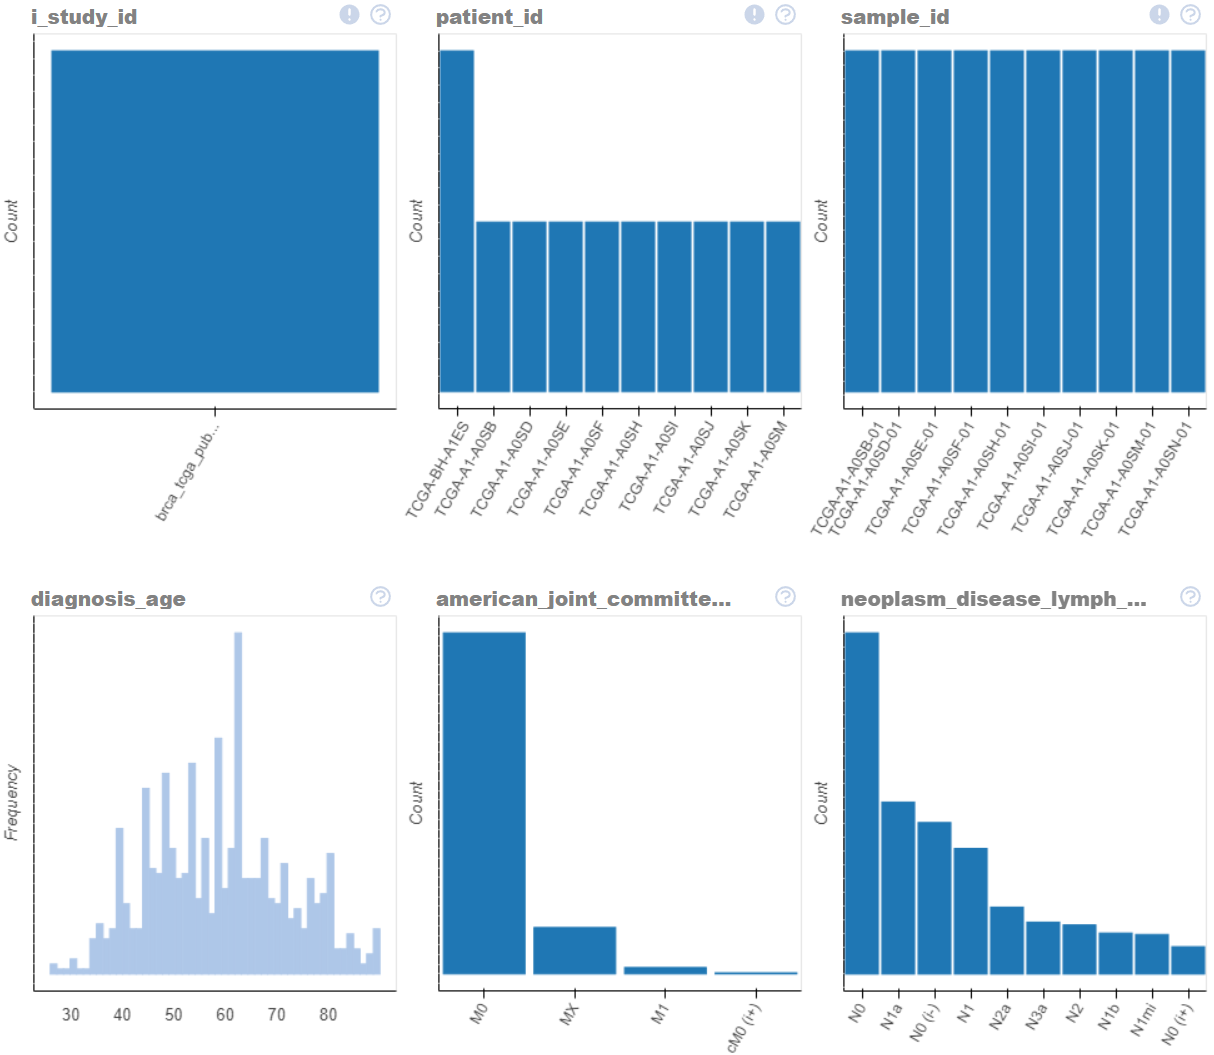
\includegraphics[width=1
	\linewidth]{NOTEBOOK/IMAGES_EDA/1}
\end{figure}

\begin{figure}
	\centering
	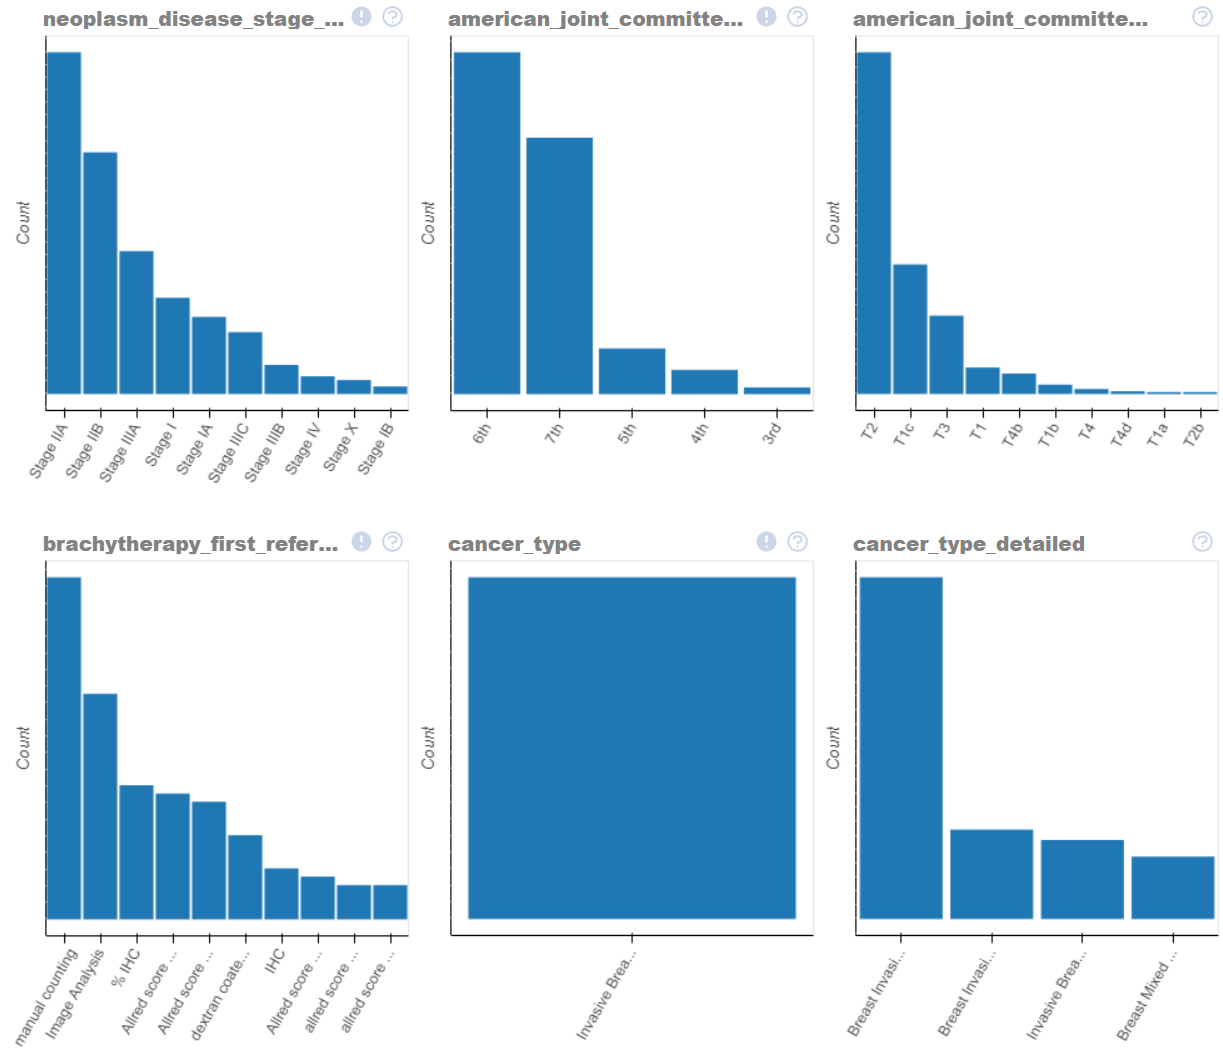
\includegraphics[width=1
	\linewidth]{NOTEBOOK/IMAGES_EDA/2}
\end{figure}

\begin{figure}
	\centering
	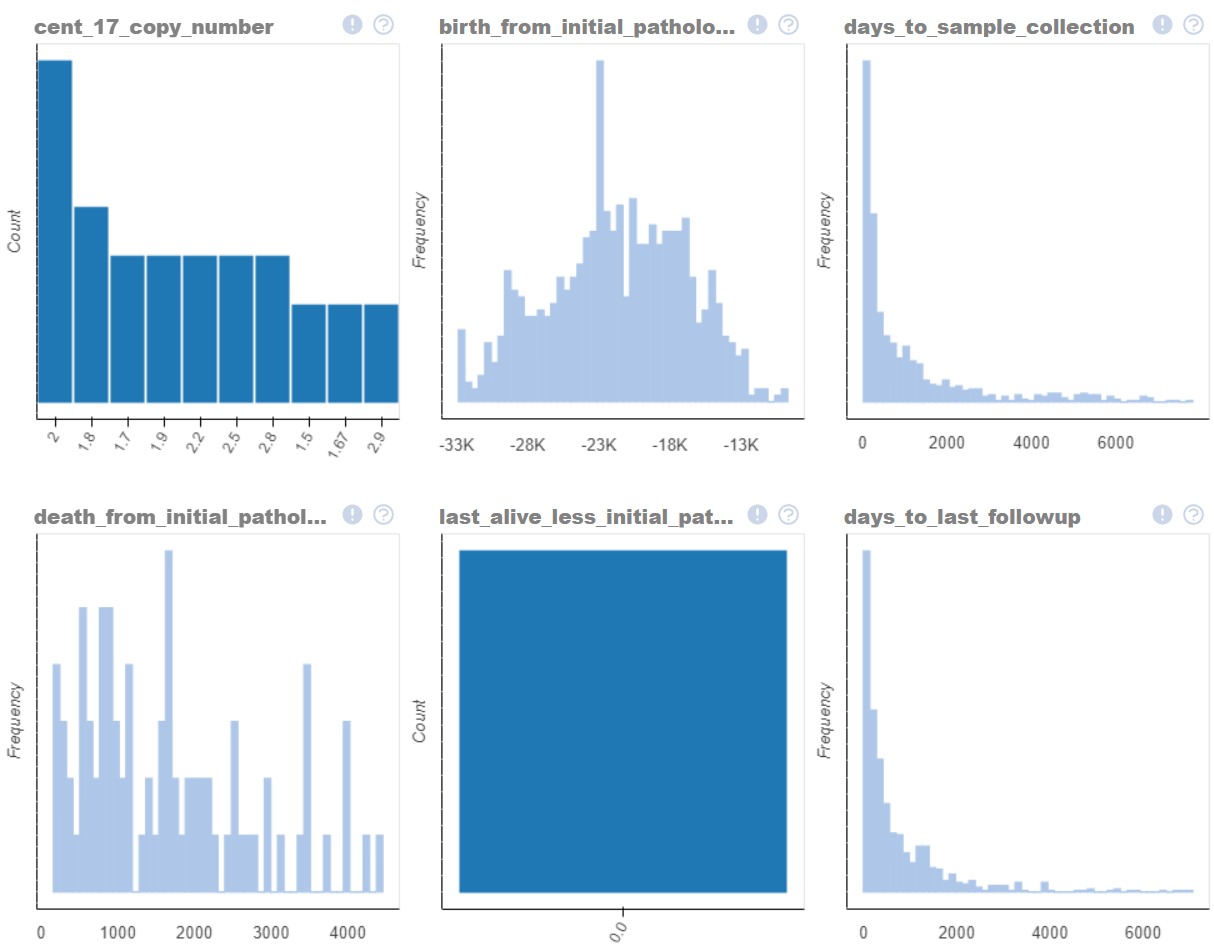
\includegraphics[width=1
	\linewidth]{NOTEBOOK/IMAGES_EDA/3}
\end{figure}

\begin{figure}
	\centering
	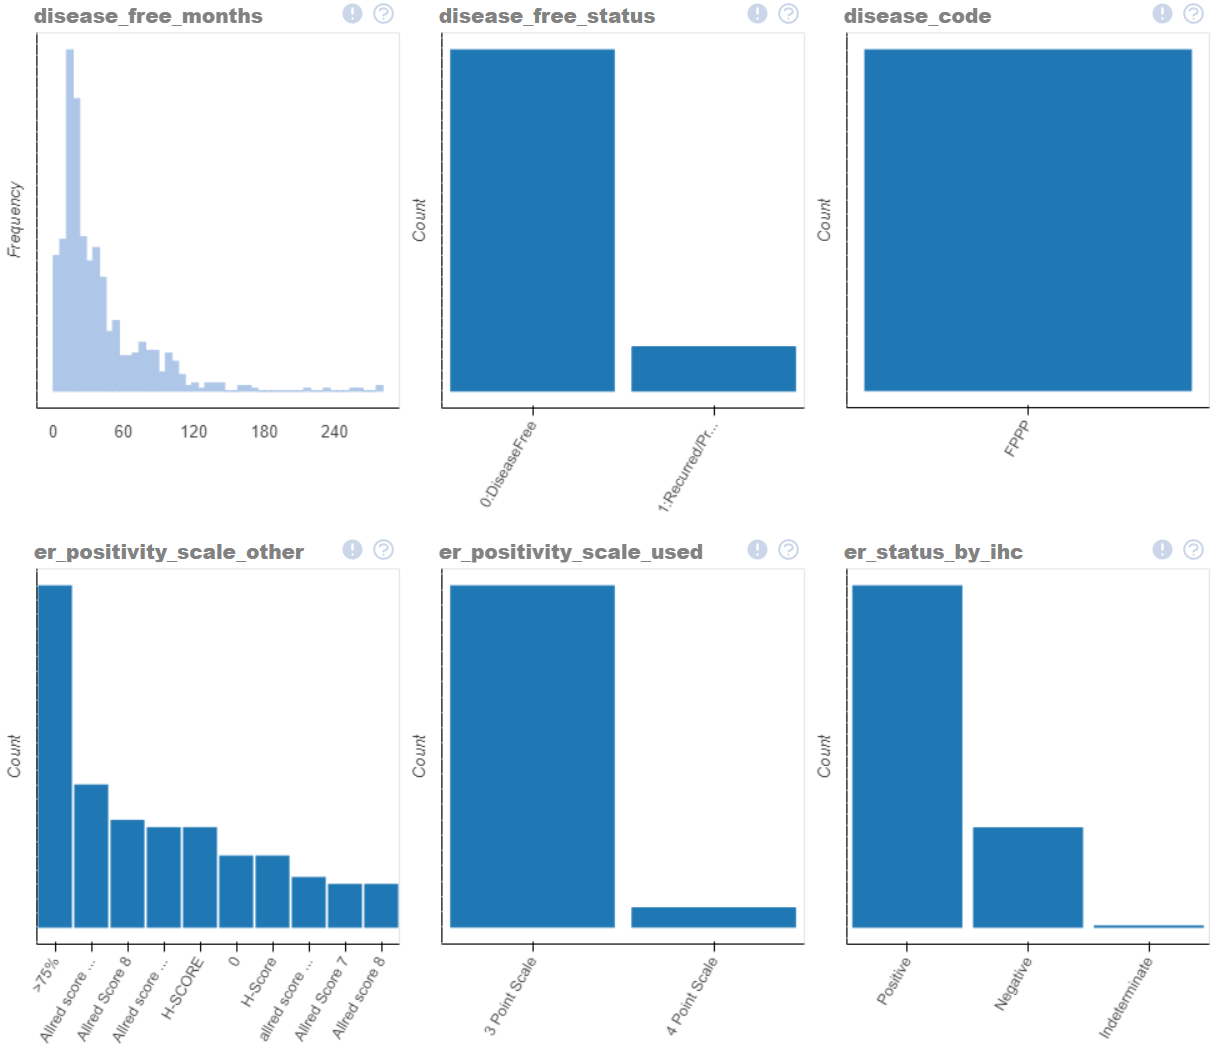
\includegraphics[width=1
	\linewidth]{NOTEBOOK/IMAGES_EDA/4}
\end{figure}

\begin{figure}
	\centering
	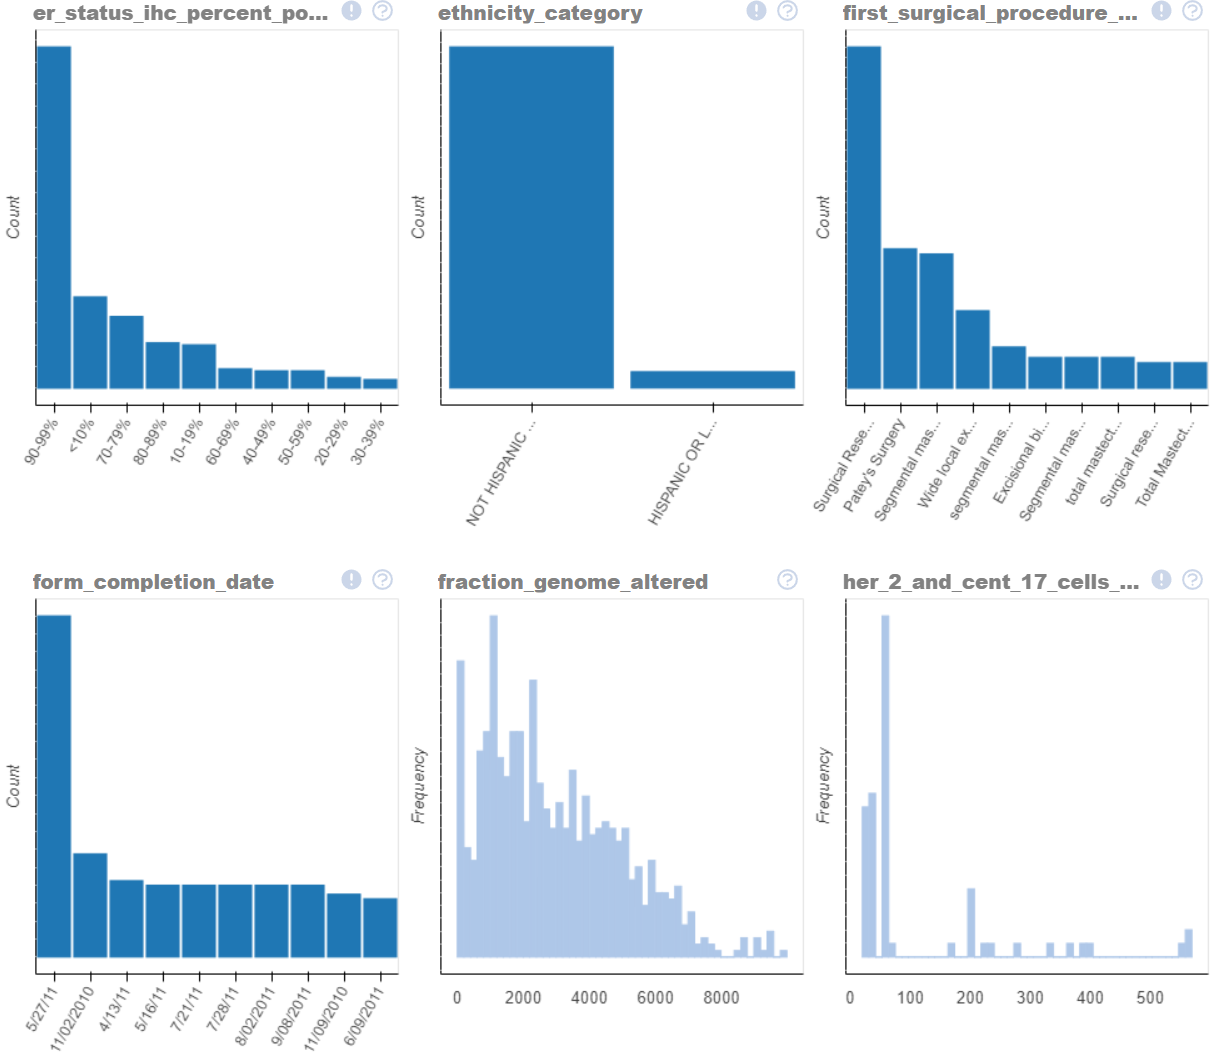
\includegraphics[width=1
	\linewidth]{NOTEBOOK/IMAGES_EDA/5}
	\label{EDA}
	\caption{Distribución del conjunto de datos del Carcinoma invasivo de mama.}\label{fig:foobar}
\end{figure}


\subsection{Detección de datos Ausentes}
En segundo lugar, basados en la obtención de los atributos del conjunto de datos \textit{“Breast Invasive Carcinoma (TCGA, Cell 2015)”}, se realizo un análisis de la cantidad de datos perdidos para identificar las variables y en la etapa posterior realizar la limpieza y el pre-procesamiento de los datos de destino hacerlos consistentes y sin ningún tipo de ruido. Los resultados obtenidos se pueden observar en la figura \ref{Missing_Bar_Chart}:


\begin{figure}[!htb]
	\centering
	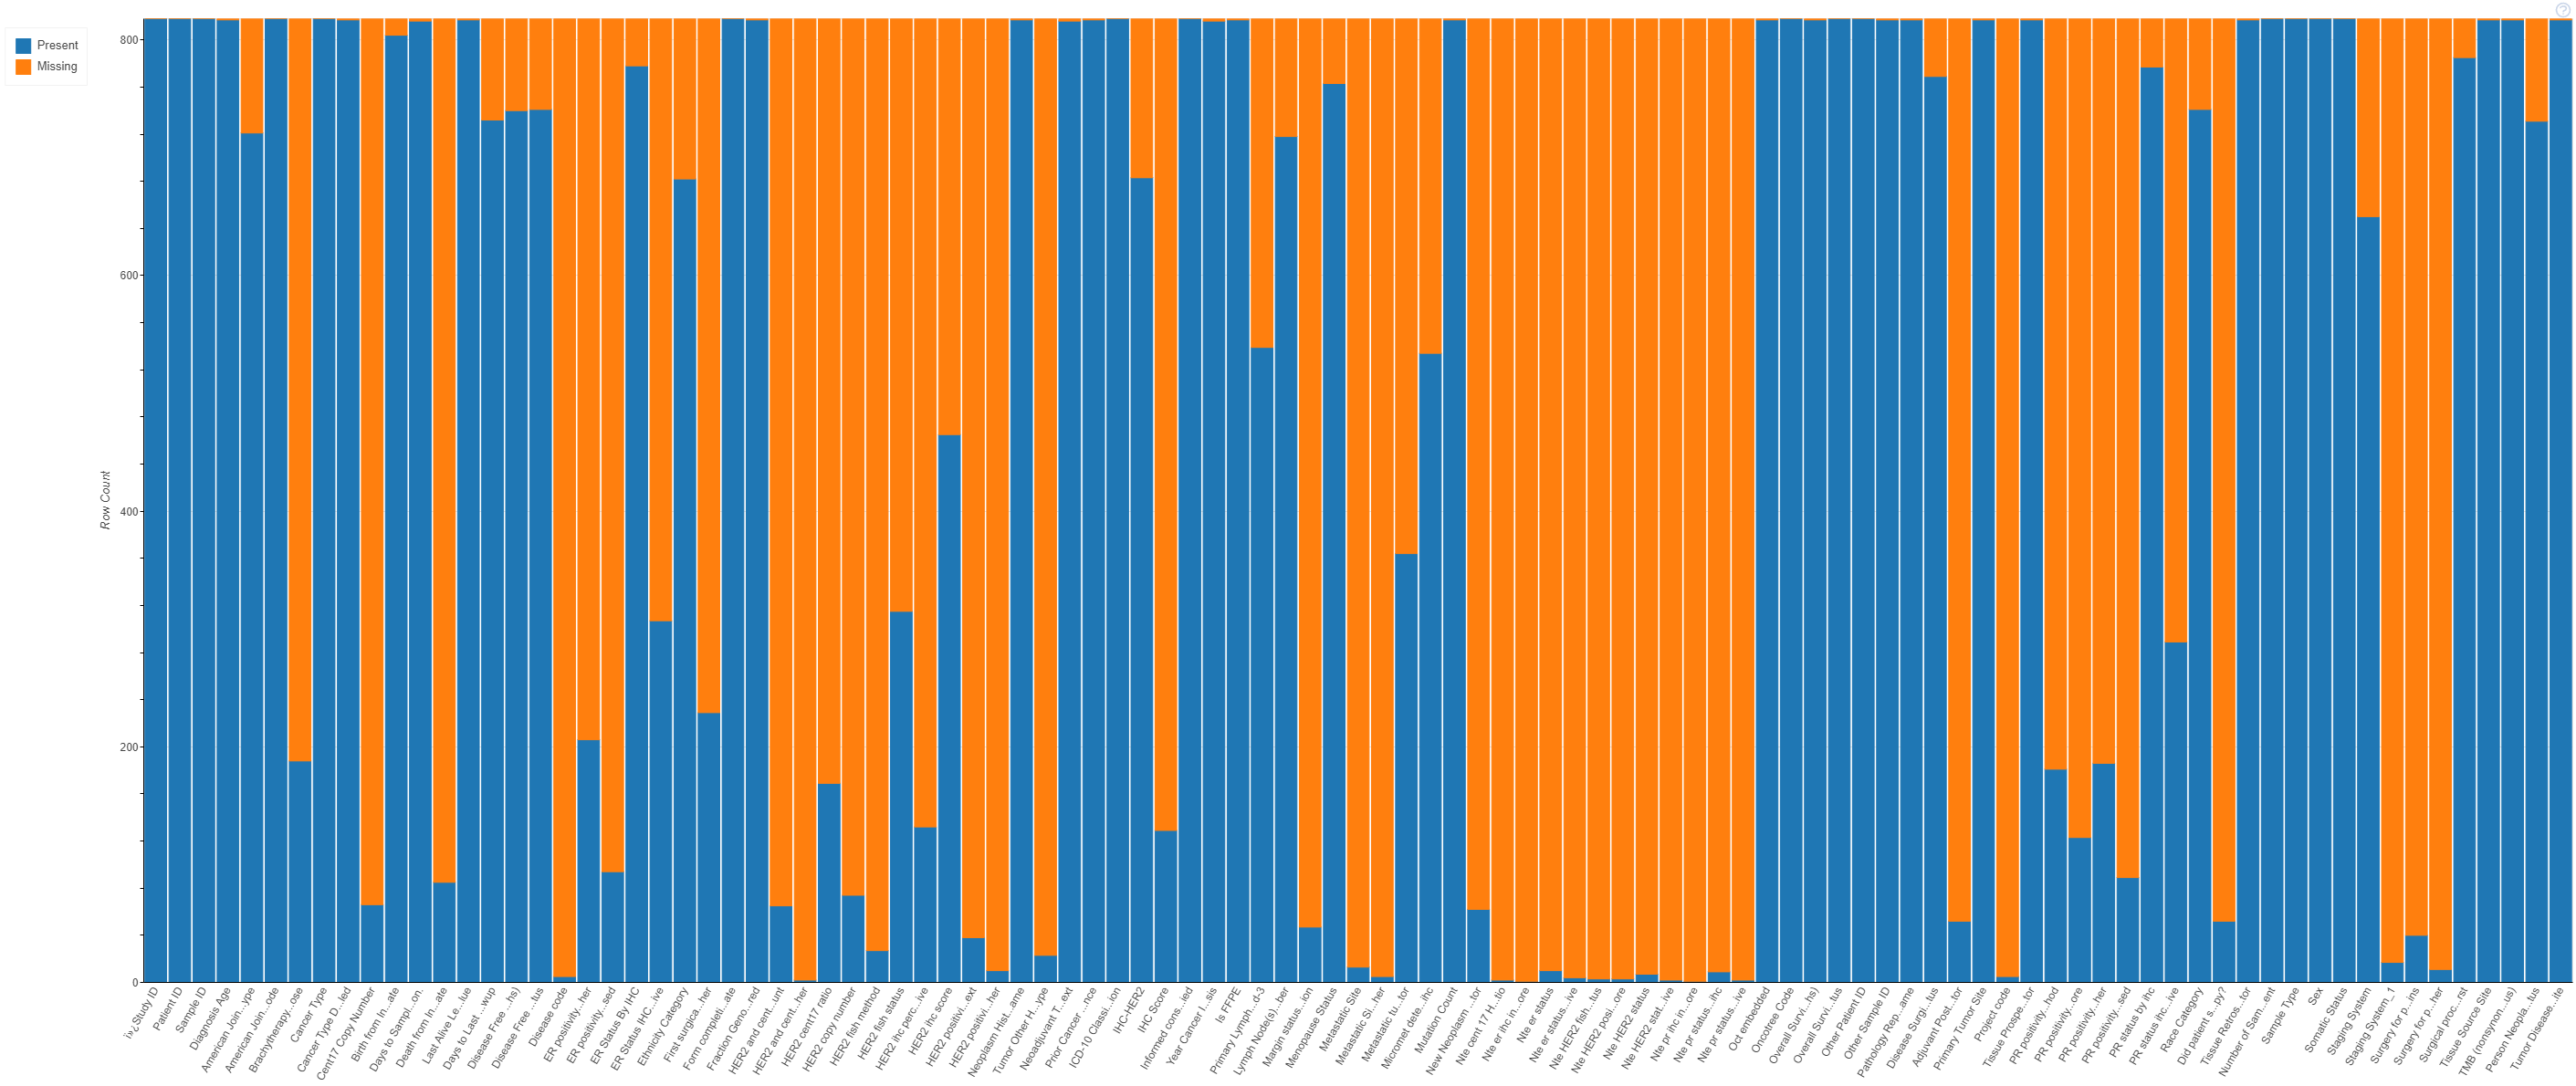
\includegraphics[width=1\linewidth]{IMAGENES/Missing_Bar_Chart}
	\caption{Datos perdidos expresados en una gráfica de barras.}
	\label{Missing_Bar_Chart}
\end{figure}

\begin{figure}[!htb]
	\centering
	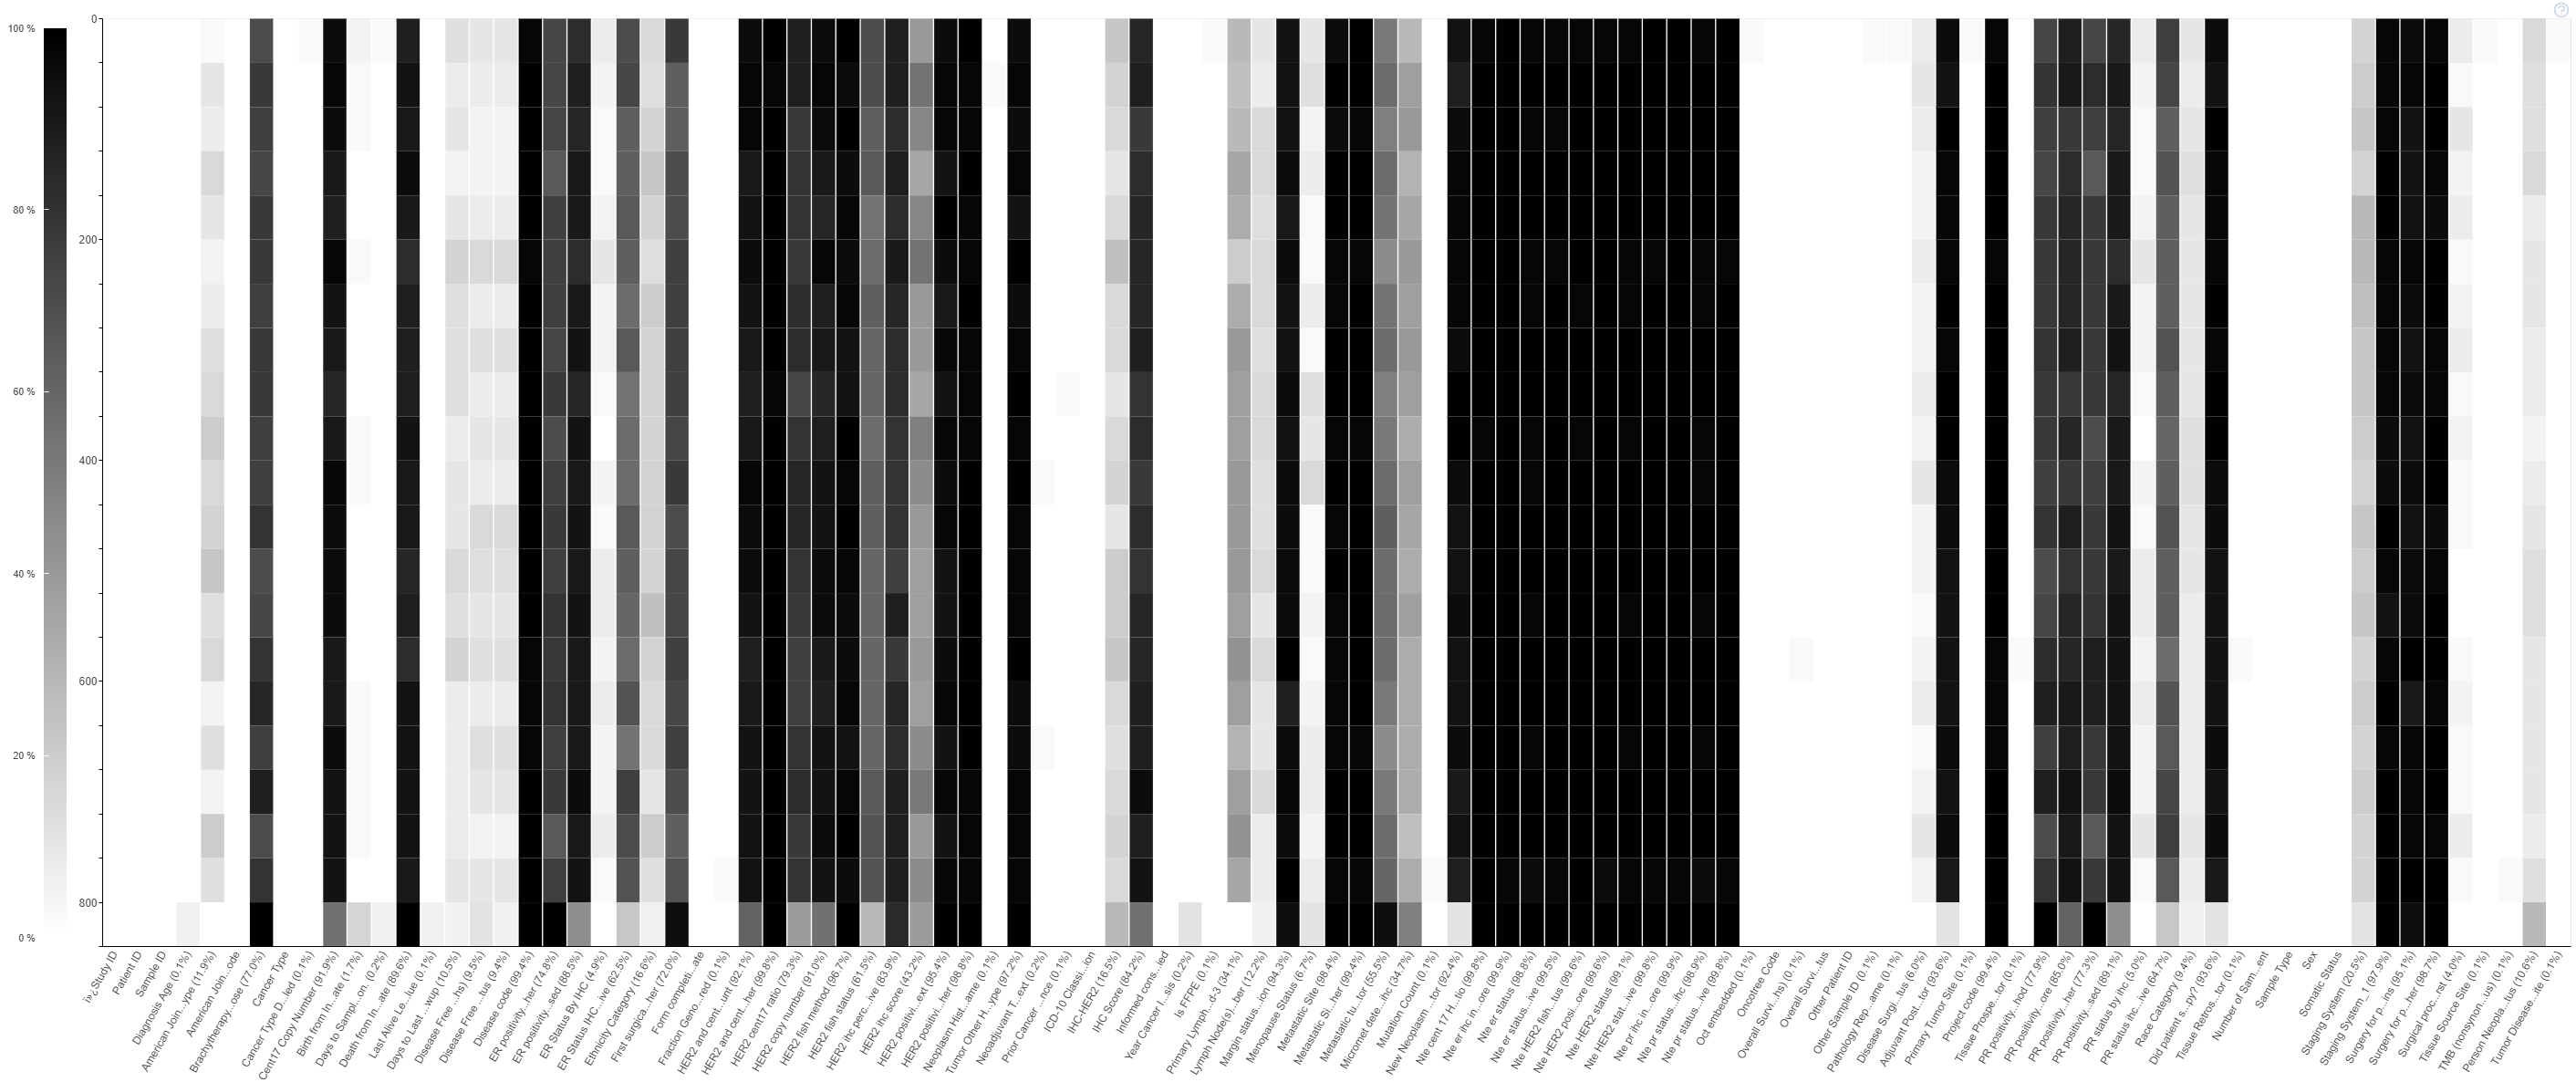
\includegraphics[width=1
	\linewidth]{IMAGENES/Missing_Spectrum}
	\caption{Datos perdidos expresados en un diagrama espectral.}
	\label{Missing_Spectrum}
\end{figure}


\subsection{Análisis Descriptivo }
En primer lugar, se realizo el respectivo análisis descriptivo para detectar cual es comportamiento de los atributos del conjunto de datos \textit{“Breast Invasive Carcinoma (TCGA, Cell 2015)”}. En la gráfica \ref{EDA} se puede observar las gráficas estadísticas unidimensionales de la 110 variables, las cuales permitieron extraer  las características mas representativas y permitieron identificar el comportamiento de los datos.

\begin{table*}[!htb]
	\footnotesize
	\begin{threeparttable}
		\caption{Conjunto de datos del Carcinoma invasivo de mama (TCGA, Cell 2015).}
		\label{Analisis_Descriptivo}
		\begin{tabular}{p{8cm} p{7cm}} \toprule	 
			\begin{center}Análisis descriptivo\end{center}             
			&\begin{center}Variable\end{center}\\ \hline
			%------------------------------------------------------	
			La \textit{edad de diagnostico} del cáncer de mama tiene una tendencia central de 59 años, en donde la edad mínima presentada es de  26 años y la edad máxima presentada es de 90 años.
			
			& \begin{center}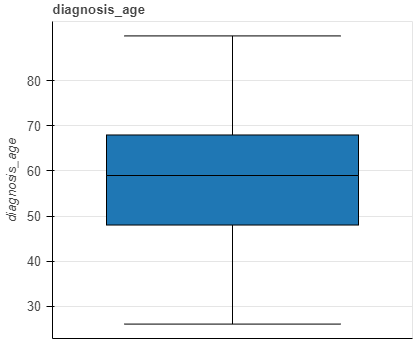
\includegraphics[width=1\linewidth]{NOTEBOOK/IMAGENES_DESCRIPTIVAS/1_diagnosis_age}\end{center}
			\\ \hline
			%------------------------------------------------------	
			El código AJCC para la \textit{estadificación metastásica(M) del cáncer} se visualiza en orden descendente de la siguiente manera: En primer lugar, el código \textit{m0} se presenta en 707 pacientes en donde el cáncer hizo metástasis pero no se  disemino a otras partes del cuerpo. En segundo lugar se encuentra el código \textit{mx} presentado en 96 pacientes a los cuales no fue posible medir la metástasis. En tercer lugar se encuentra el código \textit{m1} presentado en 13 pacientes en donde el cáncer se diseminó a otras partes del cuerpo. En ultimo lugar se encuentra el código \textit{cM0(i+)} presentado en 2 pacientes en los cuales no se detecto evidencia de metástasis a distancia, pero hubo un pequeño número de células en las cuales se encontró una metástasis diminuta (no mayor de 0.2 mm) detectada en ganglios linfáticos no regionales \cite{NCI}.
			
			& \begin{center}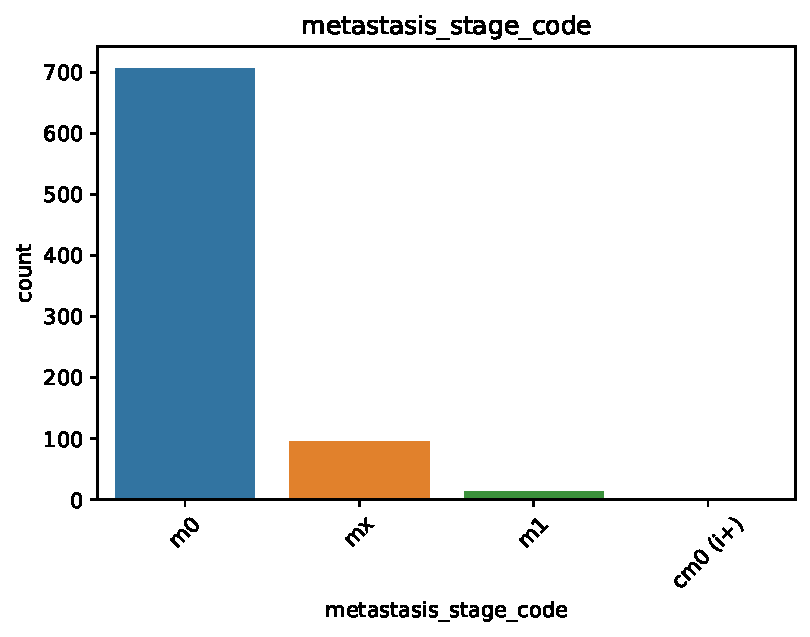
\includegraphics[width=1\linewidth]{NOTEBOOK/IMAGENES_DESCRIPTIVAS/2_metastasis_stage_code}\end{center}
			\\ \hline
			%------------------------------------------------------	
			El código AJCC para la \textit{estadificación del cáncer por neoplasia del ganglio linfático(N)} se visualiza en orden descendente de la siguiente manera: En primer lugar, el código \textit{n0} se presenta en 250 pacientes en donde no hay cáncer en los ganglios linfáticos cercanos. En segundo lugar, el código \textit{n1a} se presento en 126 pacientes en donde el cáncer se diseminó a 1 ganglio linfáticos debajo del brazo con al menos un área de cáncer diseminada de más de 2 mm de ancho. En tercer lugar el código \textit{n0(i-)} se presento en 126 pacientes en donde, no hay evidencia histológica de metástasis en los ganglios linfáticos regionales. Del cuarto lugar en adelante, se refiere a la cantidad y ubicación de los ganglios linfáticos que contienen cáncer. Cuanto mayor sea el número después de la $n$, más ganglios linfáticos se vieron afectados.	
			
			& \begin{center}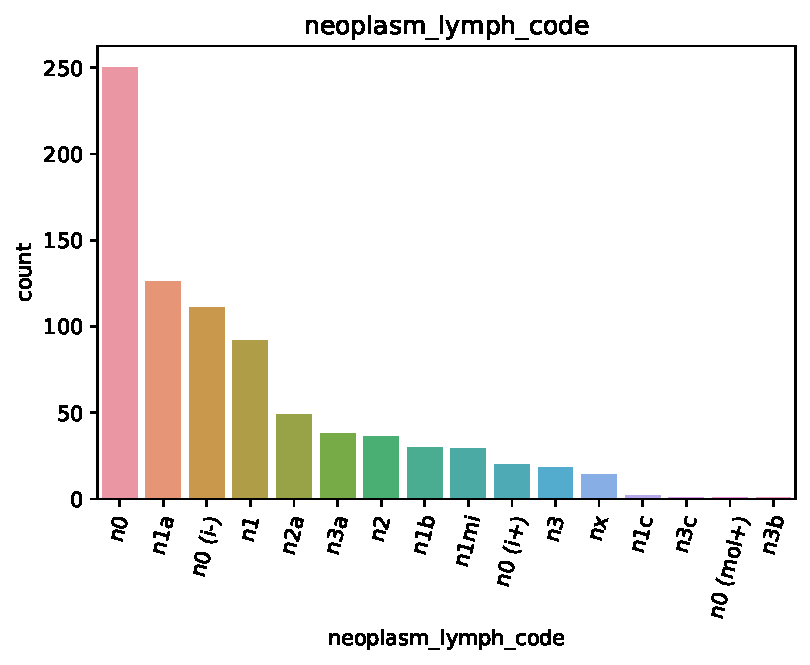
\includegraphics[width=1\linewidth]{NOTEBOOK/IMAGENES_DESCRIPTIVAS/3_neoplasm_lymph_code}\end{center}
			\\ \hline
			%------------------------------------------------------	
		\end{tabular}
	\end{threeparttable}
\end{table*}

\begin{table*}[!htb]
	\footnotesize
	\begin{threeparttable}
		\begin{tabular}{p{8cm} p{7cm}} \toprule	 
			%------------------------------------------------------	
			Las etapas AJCC para la \textit{estadificación del cáncer por neoplasia} se visualiza en orden descendente de la siguiente manera: En primer lugar, la \textit{etapa iia} se presenta en 278 pacientes en donde el tumor mide más de 20 mm pero no más de 50 mm y no se ha propagado a los ganglios linfáticos axilares. En segundo lugar, la \textit{etapa iib} se presento en 190 pacientes en donde el tumor mide más de 50 mm pero no se ha propagado a los ganglios linfáticos axilares. En tercer lugar la \textit{etapa iiia} se presento en 112 pacientes en donde el tumor se diseminó de 4 a 9 ganglios linfáticos axilares o los ganglios linfáticos mamarios internos, pero no se ha propagado a otras partes del cuerpo. En cuarto lugar, la \textit{etapa i} se presento en 75 pacientes  en donde el tumor es pequeño, invasivo y no se ha propagado a los ganglios linfáticos. En quinto lugar, la \textit{etapa ia} se presento en 60 pacientes en donde el tumor mide menos de 20 mm  y no se ha propagado a los ganglios linfáticos. Del sexto lugar en adelante, el tumor puede tener cualquier tamaño y se ha propagado a otros órganos, como los huesos, los pulmones, el cerebro, el hígado, los ganglios linfáticos distantes o la pared torácica.
			
			& \begin{center}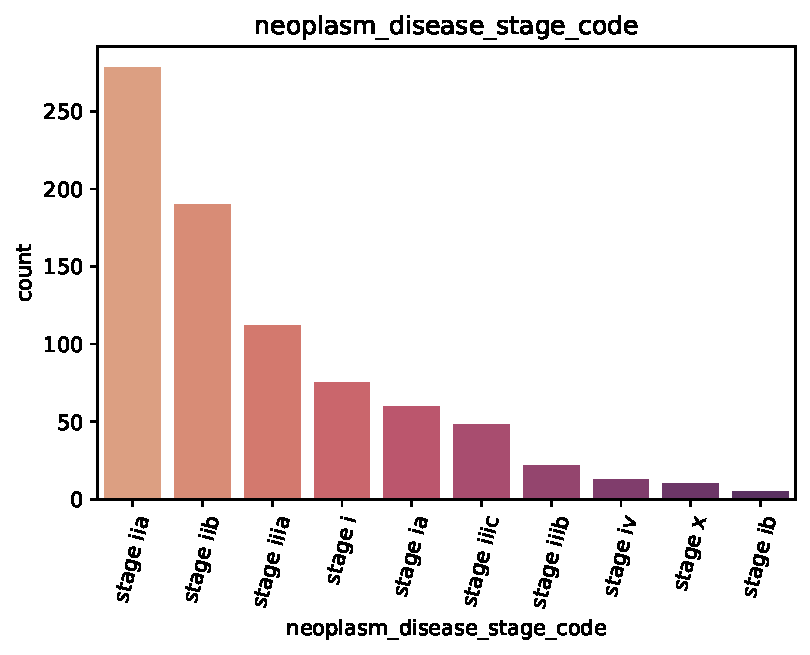
\includegraphics[width=1\linewidth]{NOTEBOOK/IMAGENES_DESCRIPTIVAS/4_neoplasm_disease_stage_code}\end{center}
			\\ \hline
			%------------------------------------------------------	
			El código AJCC para la \textit{estadificación el tumor (T) primario del cáncer} se visualiza en orden descendente de la siguiente manera: En primer lugar, el código \textit{t2} se presenta en 459 pacientes en donde el tumor mide más de 20 mm pero no más de 50 mm. En segundo lugar, el código \textit{t1c} se presento en 173 pacientes en donde el tumor mide  de 10 mm a 20 mm o menos. En tercer lugar el código \textit{t3} se presento en 104 pacientes en donde el tumor mide más de 50 mm. En cuarto lugar el código \textit{t1} se presento en 34 pacientes en donde el tumor  mide 20 mm o menos en su área más ancha. En quinto lugar el código \textit{t4b} se presento en 26 pacientes en donde el tumor ha crecido dentro de la piel. Del sexto lugar en adelante, el código \textit{t1b} se presento en 11 pacientes en donde el tumor mide más de 5 mm pero menos de 10 mm, el código \textit{t4} se presento en 5 pacientes en donde el tumor ha crecido hacia la pared torácica, el código \textit{t4d} se presento en 2 pacientes en donde es cáncer de mama inflamatorio, el código \textit{t1a} se presento en 1 paciente en donde el tumor mide más de 1 mm pero menos de 5 mm, el código \textit{t2b} se presento en 1 paciente en donde el tumor mide más de el tumor mide más de 25 mm pero menos de 50 mm.
			
			& \begin{center}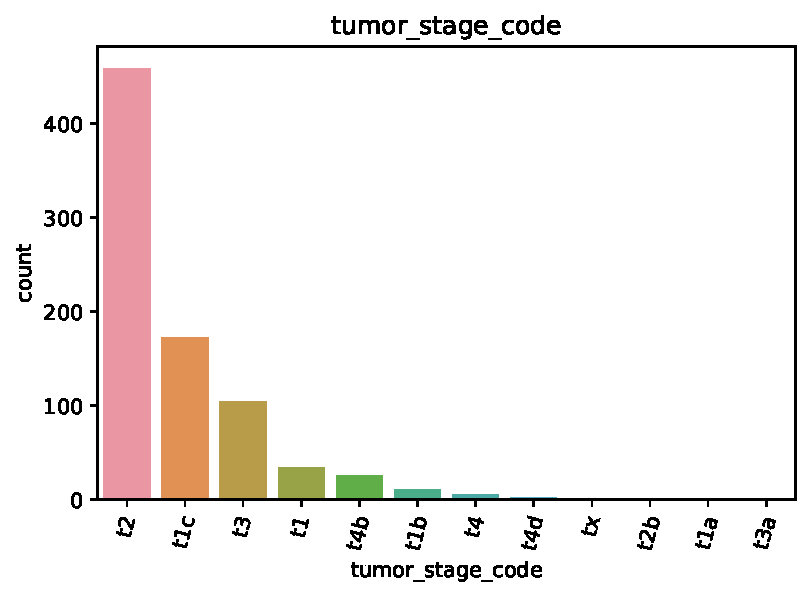
\includegraphics[width=1\linewidth]{NOTEBOOK/IMAGENES_DESCRIPTIVAS/5_tumor_stage_code}\end{center}
			\\ \hline
		\end{tabular}
	\end{threeparttable}
\end{table*}

\begin{table*}[!htb]
	\footnotesize
	\begin{threeparttable}
		\begin{tabular}{p{8cm} p{7cm}} \toprule	 
			%------------------------------------------------------	
			El \textit{tipo de cáncer de mama} se visualiza en orden descendente de la siguiente manera: En primer lugar, el \textit{cáncer Ductal invasivo} se presento en 491 pacientes. En segundo  lugar, el \textit{cáncer Lobulillar invasivo} se presento en 127 pacientes. En tercer lugar, el \textit{cáncer invasivo con otros diagnósticos} se presento en 112 pacientes. En cuarto lugar,  el \textit{cáncer mixto (Ductal y Lobulillar)} se presento en 88 pacientes.
			
			& \begin{center}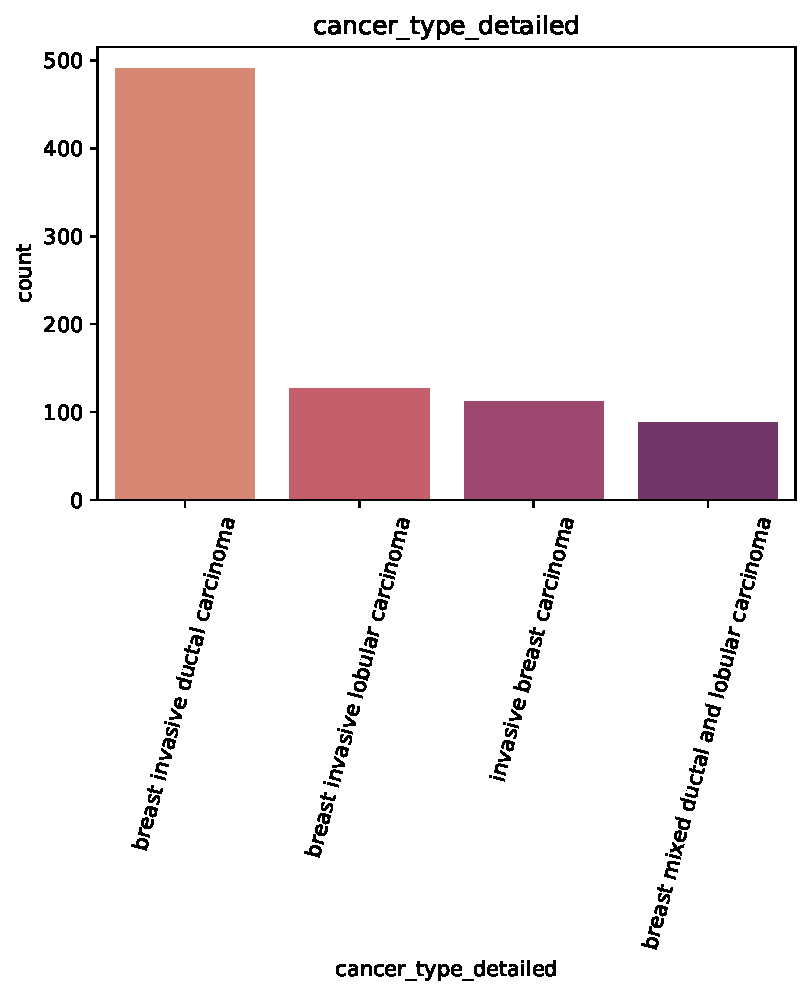
\includegraphics[width=1\linewidth]{NOTEBOOK/IMAGENES_DESCRIPTIVAS/6_cancer_type_detailed}\end{center}
			\\ \hline
			%------------------------------------------------------	
			El intervalo de días para la \textit{recolección de muestras} tiene una tendencia central aproximada de 451 días en donde el tiempo mínimo presentado es de 16 días y el tiempo máximo presentado de 7804 días.
			
			& \begin{center}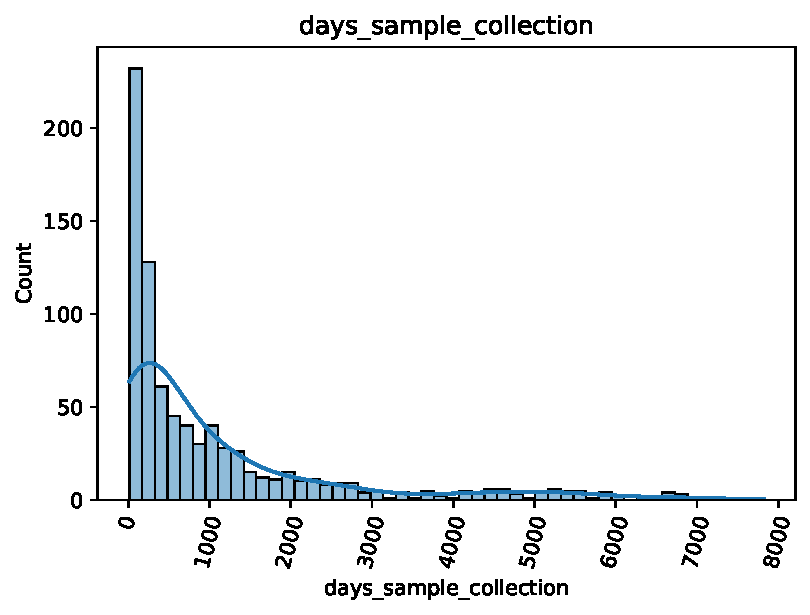
\includegraphics[width=1\linewidth]{NOTEBOOK/IMAGENES_DESCRIPTIVAS/7_days_sample_collection}\end{center}
			\\ \hline
		\end{tabular}
	\end{threeparttable}
\end{table*}









